% /******** Optymalizacja *********/
\chapter{Optymalizacja}
Do wyznaczenia optymalnych parametrów regulatorów PID i DMC użyliśmy funkcji \emph{fmincon} oraz \emph{GA}. Są to funkcje pozwalające wyznaczyć minimum (globalne) zadanej funkcji celu.
W obu przypadkach regulatorów, funkcję celu traktujemy jako suma kwadratów błędów ( między wyjściem obiektu a wartością zadaną ).
Do wyznaczenia optymalnych parametrów regulatora PID użyliśmy funkcji \emph{fmincon}. Optymalizujemy trzy parametry: K (wzmocnienie - X(1)), Ti (X(2)) oraz Td (X(3)).
Ograniczeniem jakie przyjmujemy są dodatnie wartości parametrów regulatora. Po uruchomieniu \emph{fmincon} otrzymujemy następujące parametry:
\begin{align}
  K &= 1.2958 \nonumber \\
  T_d &= 21.8912 \\
  T_i &= 4.7082 \nonumber
\end{align}
Wyniki zostały zobrazowane na wykresie \ref{fig:optim_pid}.
Zauważamy, że funkcja celu przyjmuje niższą wartość niż dla parametrów regulatora wyznaczonego metodą inżynierską, co sugeruje prawidłowe działanie funkcji optymalizacji.
\begin{figure}
  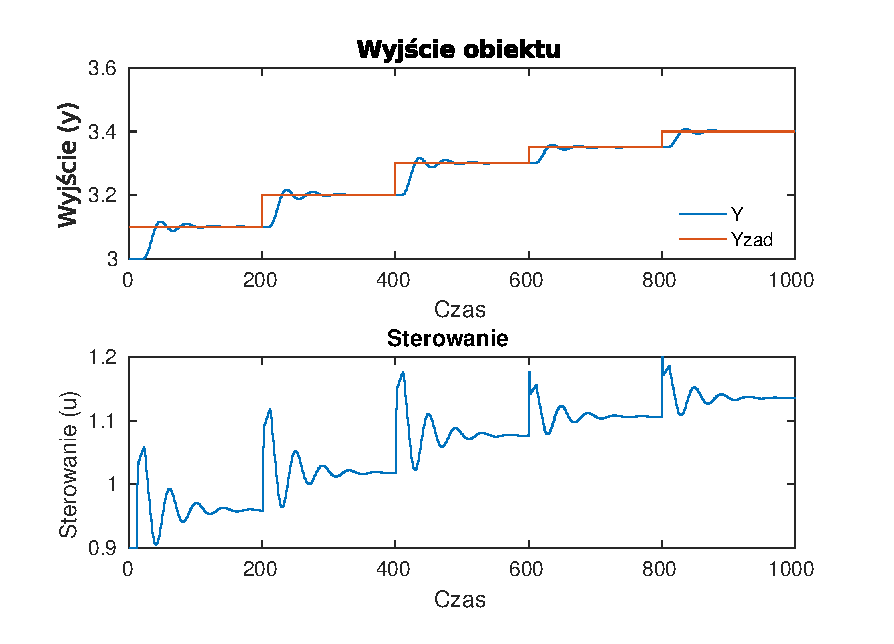
\includegraphics{wykresy/optim_pid.eps}
  \caption{Regulator PID z nastawami wyznaczonymi funkcją \emph{fmincon}.}
  \label{fig:optim_pid}
\end{figure}
Do wyznaczenia optymalnych parametrów regulatora DMC użyliśmy funkcji \emph{GA}. Jest to algorytm genetyczny umożliwiający znalezienie minimum danej funkcji. Optymalizujemy trzy parametry:
N - horyzont predykcji,
Nu - horyzont sterowania,
$\lambda$ - współczynnik 'kary' za zmiany sterowania.
Użycie algorytmu \emph{GA} motywujemy tym, że w przeciwieństwie do \emph{fmincon}, możemy wprowadzić ograniczenie na N oraz Nu, tak aby ich wartości mogły być dodatnie całkowite.
Po uruchomieniu \emph{GA} otrzymujemy następujące parametry:
\begin{align}
  N &= 74 \nonumber \\
  N_u &= 1 \\
  \lambda &= 30.2824 \nonumber
\end{align}
Wyniki obrazuje wykres \ref{fig:optim_dmc}.
Zauważamy, że funkcja celu przyjmuje niższą wartość niż dla parametrów regulatora DMC wyznaczonego na chybił trafił, oraz zdecydowanie lepsze niż parametry optymalne regulatora PID.
\begin{figure}
  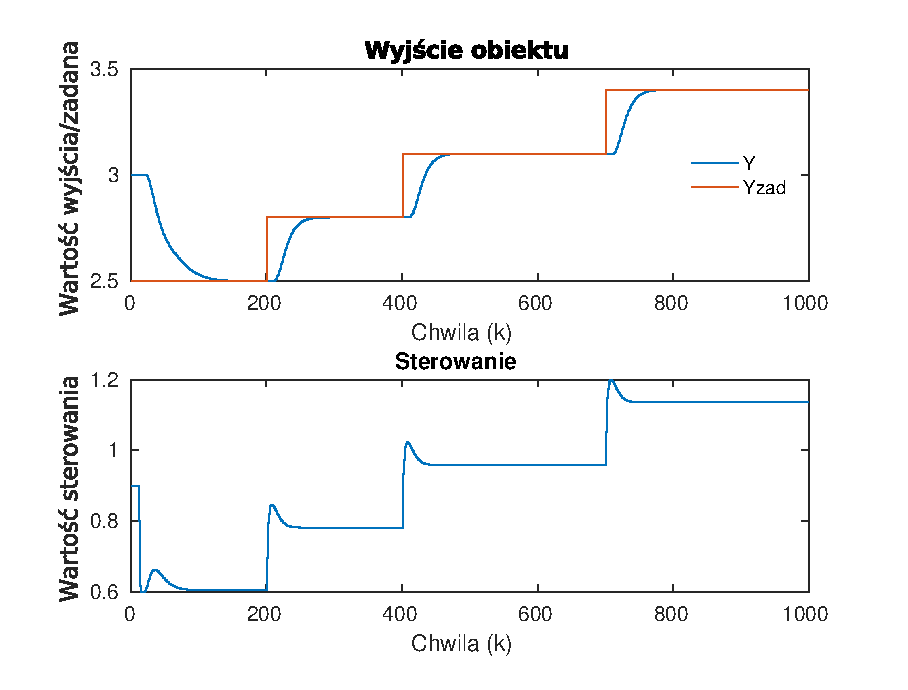
\includegraphics{wykresy/optim_dmc.eps}
  \caption{Regulator DMC z nastawami wyznaczonymi funkcją \emph{GA}.}
  \label{fig:optim_dmc}
\end{figure}
